\chapter{Routing Variants}

In Layer 3 routing, you bascially compute next hop information based on the IP destination address,
shifting the ethernet source and destination as you move the packet along.  In routing, you 
always keep the remaining header values, especially the IP source and destination address, 
constant. 

A few useful variants of Layer 3 routing change other packet headers as well:

\begin{itemize}
\item In \emph{load balancing}, a few servers with different IP addresses can act as exact copies
of on another.  A single artificial IP address, called the \emph{front-end} IP, is where clients send their
packets, and a load balancer changes the front-end IP to a real server IP as it moves the packet.
Ths load balancer can partition user traffic to maximize efficiency.
\item In \emph{network address translation}, or NAT, a group of client machines share a single
externally visible, public IP address.  But the machines themselves use private, non-routable
IP addresses.  The NAT box translates these private addresses to the public one on outgoing packets,
and the reverse on incoming ones.   NAT enables conversations originating on the private
network only, and blocks conversations originating outside the private network.  
\item In a \emph{firewall}, NAT is augmented with security features to allow incoming traffic
as well.  The traffic must follow certain rules -- for example, only port 80 on a certain IP.  
\end{itemize}

In this chapter, we'll write a load balancer.  The concepts are applicable to other 
types of routing devices.  

In previous chapters, we always wrote our programs from a blank slate.  Because load balancers, 
NAT boxes and firewalls are so much like routing, we will take a different approach.  We will
treat the router handler as a superclass, and write our specialized device as a subclass of it.
In addition, we'll use the NIB developed for routers and subclass it to add any additional 
information needed for the specialized box.  

Object oriented concepts in something new that SDN brings to the table.  With hardware-based
traditional network devices, you could only extend them in ways the vendor allowed.  This is 
like the days of canned, non object-oriented software -- changing the behavior of small 
parts was virtually impossible without the source code.  With Frenetic, you can build a library
of easily extendible network pieces, and use them for purposes far beyond what the original
authors intended. 

\section{Design}

A \emph{load balancer} distributes client requests to certain servers invisibly.  When
we enter a request to http://www.google.com, which is one IP address, the request is handled
by one of thousands of servers at Google.  This is good for the client, who then doesn't have to 
try certain backend IP addresses until they find a fast server.  But it's also good for the 
server owner's security -- by not publicly posting their back end IP's, they can prevent 
coordinated attacks on certain servers.  (Of course, you can attack the load balancer, but 
this box usually has more intelligence to detect such things).  

So let's take a small example.  In the following network:

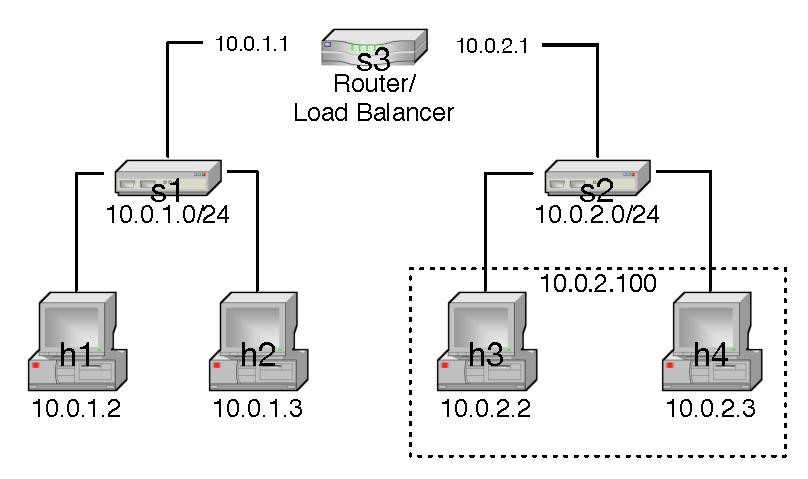
\includegraphics{load_balancing_topo.pdf}

Clients in the 10.0.1.0/24 network issue a request to 10.0.2.100, called the \emph{front-end IP}.
No actual host owns this front-end IP, and network administrators must take steps to assure
it's not re-used by some real host.  The IP's of the two hosts in the 10.0.2.0/24 network: 
h3 at 10.0.2.2 and h4 at 10.0.2.3 are called \emph{back-end IP's}.  In our example,
h3 and h4 are exact equivalents, and can service the same set of requests.  It doesn't matter
which host serves the content.  

We use this information to power the load balancer.  So if h3 and h4 are equivalent, how
does the load balancer decide where to send a request for 10.0.2.100?  The load balancer
can be as simple or as sophisticated as you want:

\begin{itemize}
\item In \emph{Round Robin} scheduling, each subsequent request goes to the next server in the 
chain.  The first goes to h3, the second to h4, the third back to h3, and so on.  
\item In \emph{Sticky Round Robin}, clients are assigned to a server on first request.  So 
if h2 asks for 10.0.2.100 first, it will be assigned to h3.  Subsequent requests from h2
will continue to go to h3.  A request from h1 might then go to h4.  
\item In \emph{Least Utilized}, each request is assigned the server that has the lowest 
utilization by some measure (least CPU usage, least network traffic, etc.)
\end{itemize}

Different network applications benefit from different strategies.  For example, web apps that
use server-side state tend to use Sticky Round Robin.  This assures that subsequent requests
from a client can access the same server-side state without complex state-distribution 
mechansims.  Applications that have heavy CPU usage like reporting benefit from a Least Utilized
strategy.  This prevents someone with a long-running report from slowing down the system 
unnecessarily for others with short requests.

With SDN, you can write arbitrarily complex load balancing algorithms.  For our example,
we will use Sticky Round Robin.  A Load Balancer must do three things:

\begin{itemize}
\item When the first request comes in, it must select a back-end IP to rewrite.  It notes this
in a table.
\item It then rewrites the packet with the back-end IP, does the typical routing thing of 
altering the MAC addresses, and forwards the packet.  It must do this because the back end host
must receive a request bound for its own IP - if it receives one for 10.0.2.100, it'll simply drop
the packet.
\item Lastly, when the reply comes, it must reverse the step.  It rewrites the source IP back to 
the front-end IP 10.0.2.100, then does the typical routing thing.   If it does not do this, the 
host will receive a reply from a back-end IP, which it never sent to, and will probably drop
the packet.  
\end{itemize}

\section{Implementation}

So let's get to it!  In the first incarnation of or load balancer, as in the past, we'll 
do load balancing tasks solely in the controller.  Once that's debugged, we can move these
steps to rules in the flow table.  To configure the load balancer, as in the past
we'll use a JSON file.  

Here's one for our sample network, from \codefilename{routing_variants/load_balancer.json}:

\inputminted{python}{code/routing_variants/load_balancer.json}

Our Network Information Base will use the router's NIB as a 
superclass, and add load balancing attributes.   The main addition is a map of back-end IP's
to clients, and a pointer to the ``current'' back-end IP entry.  

The following code is in from \codefilename{routing_variants/load_balancer_nib.py}:

\inputminted{python}{code/routing_variants/load_balancer_nib.py}

Note how we define a subclass of Routing's \python{NetworkInformationBase} class, which
Python finds by the addition of \codefilename{../routing} to the class path.    

The method \python{backend_ip} does the heavy lifting of assigning a client IP to a back-end
server (if it hasn't already been assigned).  If this were a more sophisticated load balancing
algorithm, this method would bear the brunt of it.  Our version is fairly simple.

The following code is in from 
\codefilename{routing_variants/load_balancer1.py}:

\inputminted{python}{code/routing_variants/load_balancer1.py}

This main application uses similar techniques as the Routing main application.  It delegates
the Packet In handler, for example, to the packet-in handlers of the Switches and Load Balancer.
It uses the switch mechanism from the Routing application verbatim -- no changes are
necessary.  

One interesting addition is to the \python{connected()} handler.  Here the load balancer
handler will do some extra setup work.  When a load balancer routes a first request, it 
calculates the back-end IP, but it must also know the MAC address of that back-end IP 
(because the load balancer is also a router).  It could just flood the request to all
back-end hosts, but that could cause security problems.  Instead, the load balancer attempts
to calculate these MAC addresses up front.  In a more sophsticated load balancer, it could
also ask all back-end hosts ``are you up?'' and remove back-end hosts from the pool that are not.
In our simple case, we'll just send an ARP request to all back-end hosts and hope-for-the-best.

The following code is in from 
\codefilename{routing_variants/load_balancer_handler.py}:

\inputminted[lastline=17]{python}{code/routing_variants/load_balancer_handler.py} 

Like the load balancer NIB, \python{LoadBalancerHandler} subclasses the equivalent functionality
from the Routing handler.  That way it can override what it needs to and delegate the rest.

So the load balancer sends out ARP requests to all back-end IP's.  It does not bother 
waiting for the response -- when the hosts respond, the MAC and port will be learned as if it
were any other host.  Note that this code uses the ARP request methods from the router -- there's
no need to rewrite those.

The load balancer must intercept traffic to the front-end IP, or from the back-end IP's.  But the
router already handles this traffic natively, so we can't \netkat{Union} these rules in.   Instead
we use an \netkat{IfThenElse} to split out the traffic.  

\inputminted[firstline=19,lastline=30]{python}{code/routing_variants/load_balancer_handler.py} 

The \python{policy} method here overrides the one in \python{routing_handler}.  So load balanced
IP traffic is sent to the controller,  and the rest is delegated back to the IP or ARP handling
policies of the router.  Lastly, the \python{packet_in} handler:

\inputminted[firstline=32]{python}{code/routing_variants/load_balancer_handler.py} 

Does the heavy lifting of rewriting the IP's.  Note that we have fail-safe mechanisms in place
just in case we don't know the MAC for the back-end IP.  In this case, we send out an ARP request
and drop the packet (TCP will re-send the request, and hopefully we'll have the MAC and port
learned by then).  Non-load-balanced traffic is delegated to the Packet In handler of the
router.  

So how does this work?  Let's first start up our custom topology from the routing chapter:

\begin{minted}{console}
frenetic@ubuntu-1404:~/manual/programmers_guide/code$ cd routing
frenetic@ubuntu-1404:~/manual/programmers_guide/code/routing$ sudo python mn_dot_topology.py
*** Removing excess controllers/ofprotocols/ofdatapaths/pings/noxes
killall controller ofprotocol ofdatapath ping nox_core lt-nox_core ovs-openflowd ...
killall -9 controller ofprotocol ofdatapath ping nox_core lt-nox_core ...
pkill -9 -f "sudo mnexec"
*** Removing junk from /tmp
rm -f /tmp/vconn* /tmp/vlogs* /tmp/*.out /tmp/*.log
*** Removing old X11 tunnels
*** Removing excess kernel datapaths
ps ax | egrep -o 'dp[0-9]+' | sed 's/dp/nl:/'
***  Removing OVS datapaths
ovs-vsctl --timeout=1 list-br
ovs-vsctl --if-exists del-br s1 -- --if-exists del-br s2 -- --if-exists del-br s_router
ovs-vsctl --timeout=1 list-br
*** Removing all links of the pattern foo-ethX
ip link show | egrep -o '([-_.[:alnum:]]+-eth[[:digit:]]+)'
ip link show
*** Killing stale mininet node processes
pkill -9 -f mininet:
*** Shutting down stale tunnels
pkill -9 -f Tunnel=Ethernet
pkill -9 -f .ssh/mn
rm -f ~/.ssh/mn/*
*** Cleanup complete.
Unable to contact the remote controller at 127.0.0.1:6633
Network ready
Press Ctrl-d or type exit to quit
mininet>
\end{minted}

And then start up Frenetic, and our load balancer application.  
First we'll use h2 to ping our front-end IP.
This will be assigned our first back-end IP, 10.0.2.3.  Then we'll ping it from h1, which is
assigned to the other back-end IP, 10.0.2.2.

\begin{minted}{console}
mininet> h2 ping -c 1 10.0.2.100
PING 10.0.2.100 (10.0.2.100) 56(84) bytes of data.
64 bytes from 10.0.2.100: icmp_seq=1 ttl=64 time=85.9 ms

--- 10.0.2.100 ping statistics ---
1 packets transmitted, 1 received, 0% packet loss, time 0ms
rtt min/avg/max/mdev = 85.960/85.960/85.960/0.000 ms
mininet> h1 ping -c 1 10.0.2.100
PING 10.0.2.100 (10.0.2.100) 56(84) bytes of data.
64 bytes from 10.0.2.100: icmp_seq=1 ttl=64 time=328 ms
1 packets transmitted, 1 received, 0% packet loss, time 0ms
rtt min/avg/max/mdev = 85.960/85.960/85.960/0.000 ms
mininet>
\end{minted}

Note that our ping requests don't mention any of the back-end IP's.  The client doesn't 
even know they exist.  But the log shows evidence that they're being rerouted to different
hosts:

\begin{minted}{console}
frenetic@ubuntu-1404:~/manual/programmers_guide/code/routing_variants$ python load_balancer1.py
Starting the tornado event loop (does not return).
2016-06-09 11:42:31,831 [INFO] Connected to Frenetic - Switches: {282574488338432: [2, 1], 
  282574488338433: [2, 1, 3], 282574488338434: [2, 1, 3]}
2016-06-09 11:42:31,832 [INFO] Pausing 2 seconds to allow rules to be installed
2016-06-09 11:42:33,832 [INFO] Sending out ARP Requests to all Backend IPs
2016-06-09 11:42:33,833 [INFO] Sending out ARP Request for IP 10.0.2.3
2016-06-09 11:42:33,834 [INFO] Sending out ARP Request for IP 10.0.2.2
2016-06-09 11:42:33,843 [INFO] Learning: None/02:02:02:02:02:02 attached to ( 282574488338434 , 3 )
2016-06-09 11:42:33,889 [INFO] Learning: 10.0.2.3/00:00:02:00:00:03 attached to ( 282574488338434 , 2 )
2016-06-09 11:42:33,929 [INFO] Learning: 10.0.2.2/00:00:02:00:00:02 attached to ( 282574488338434 , 1 )
2016-06-09 11:42:33,934 [INFO] ARP reply from 10.0.2.3 for 10.0.2.1 ignored.
2016-06-09 11:42:33,975 [INFO] ARP reply from 10.0.2.2 for 10.0.2.1 ignored.
...
2016-06-09 11:42:55,592 [INFO] Rerouting request for 10.0.2.100 to 10.0.2.3/00:00:02:00:00:03
2016-06-09 11:42:55,592 [INFO] Using subnet on router port 2 mac 02:02:02:02:02:02
2016-06-09 11:42:55,640 [INFO] Rewriting reply from 10.0.2.3 to 10.0.2.100
...
2016-06-09 11:43:20,753 [INFO] Rerouting request for 10.0.2.100 to 10.0.2.2/00:00:02:00:00:02
2016-06-09 11:43:20,754 [INFO] Using subnet on router port 2 mac 02:02:02:02:02:02
2016-06-09 11:43:20,800 [INFO] Rewriting reply from 10.0.2.2 to 10.0.2.100
\end{minted}

And a quick check of the statistics in both back end hosts bears that out:

\begin{minted}{console}
mininet> h3 ifconfig
h3-eth0   Link encap:Ethernet  HWaddr 00:00:02:00:00:02
          inet addr:10.0.2.2  Bcast:10.0.2.255  Mask:255.255.255.0
          UP BROADCAST RUNNING MULTICAST  MTU:1500  Metric:1
          RX packets:1 errors:0 dropped:0 overruns:0 frame:0
          TX packets:1 errors:0 dropped:0 overruns:0 carrier:0
          collisions:0 txqueuelen:1000
          RX bytes:420 (420.0 B)  TX bytes:378 (378.0 B)

mininet> h4 ifconfig
h4-eth0   Link encap:Ethernet  HWaddr 00:00:02:00:00:03
          inet addr:10.0.2.3  Bcast:10.0.2.255  Mask:255.255.255.0
          UP BROADCAST RUNNING MULTICAST  MTU:1500  Metric:1
          RX packets:1 errors:0 dropped:0 overruns:0 frame:0
          TX packets:1 errors:0 dropped:0 overruns:0 carrier:0
          collisions:0 txqueuelen:1000
          RX bytes:518 (518.0 B)  TX bytes:476 (476.0 B)
\end{minted}

\section{A More Efficient Implementation}

OK, so this works fine, but it forces all load balancer traffic through the controller.  We can
now enshrine these actions in rules.  A simple change to our \python{policy} handler will take
care of that.  

The following code is in from 
\codefilename{routing_variants/load_balancer_handler2.py}:

\inputminted[firstline=75,lastline=85]{python}{code/routing_variants/load_balancer_handler2.py} 

First we split the load balanced cases in two: one for assigned clients, and one for not-yet-assigned
clients.  The predicate for assigned clients as in two cases: the request case and the response case 
(here we assume all requests come from a client and go to a frontend IP, and all replies are the
reverse direction):

\inputminted[firstline=19,lastline=27]{python}{code/routing_variants/load_balancer_handler2.py} 

We factor out the request and response policies from the Packet In procedure into their own methods.

\inputminted[firstline=29,lastline=52]{python}{code/routing_variants/load_balancer_handler2.py} 

And that way we can use them both in the new rules:

\inputminted[firstline=54,lastline=68]{python}{code/routing_variants/load_balancer_handler2.py} 

and in the Packet Out command of the Packet In handler:

\inputminted[firstline=87]{python}{code/routing_variants/load_balancer_handler2.py} 

\section{Summary}

Load Balancers act at Layer 3, much like a router, so we steal router functionality by 
subclassing the router and its NIB.  Then our code simply overrides router functionality
where it differs from routers - for example, in answering ARPs to the front end IP.  

To build a NAT device or firewall, you can use the same approach.  Firewalls tend to 
add functionality at layer 4 as well, looking at TCP and UDP streams as entire
conversations.  

Modern network devices gather lots of statistics about their operation, and Frenetic can
tap into these statistics.   The next chapter will show you how.  

